\PassOptionsToPackage{unicode}{hyperref}
\PassOptionsToPackage{naturalnames}{hyperref}

\documentclass[14pt]{beamer}

\mode<presentation> {

% The Beamer class comes with a number of default slide themes
% which change the colors and layouts of slides. Below this is a list
% of all the themes, uncomment each in turn to see what they look like.

%\usetheme{default}
%\usetheme{AnnArbor}
%\usetheme{Antibes}
%\usetheme{Bergen}
%\usetheme{Berkeley}
%\usetheme{Berlin}
%\usetheme{Boadilla}
%\usetheme{CambridgeUS}
%\usetheme{Copenhagen}
%\usetheme{Darmstadt}
%\usetheme{Dresden}
%\usetheme{Frankfurt}
%\usetheme{Goettingen}
%\usetheme{Hannover}
%\usetheme{Ilmenau}
%\usetheme{JuanLesPins}
%\usetheme{Luebeck}
%\usetheme{Madrid}
%\usetheme{Malmoe}
%\usetheme{Marburg}
%\usetheme{Montpellier}
%\usetheme{PaloAlto}
%\usetheme{Pittsburgh}
%\usetheme{Rochester}
%\usetheme{Singapore}
%\usetheme{Szeged}
%\usetheme{Warsaw}

% As well as themes, the Beamer class has a number of color themes
% for any slide theme. Uncomment each of these in turn to see how it
% changes the colors of your current slide theme.

%\usecolortheme{albatross}
%\usecolortheme{beaver}
%\usecolortheme{beetle}
%\usecolortheme{crane}
%\usecolortheme{dolphin}
%\usecolortheme{dove}
%\usecolortheme{fly}
%\usecolortheme{lily}
%\usecolortheme{orchid}
%\usecolortheme{rose}
%\usecolortheme{seagull}
%\usecolortheme{seahorse}
%\usecolortheme{whale}
%\usecolortheme{wolverine}

%\setbeamertemplate{footline} % To remove the footer line in all slides uncomment this line
%\setbeamertemplate{footline}[page number] % To replace the footer line in all slides with a simple slide count uncomment this line

\setbeamertemplate{navigation symbols}{} % To remove the navigation symbols from the bottom of all slides uncomment this line
\setbeamertemplate{frametitle continuation}[from second][\insertcontinuationtext]
}

\usepackage{graphicx} % Allows including images
\usepackage{booktabs} % Allows the use of \toprule, \midrule and \bottomrule in tables
\usepackage[T1]{fontenc}
\usepackage[spanish]{babel}
\usepackage[utf8]{inputenc}
\usepackage{listings}
\usepackage{tikz}
\usetikzlibrary{positioning,backgrounds}
\usetikzlibrary{decorations.pathmorphing,math}
%\usepackage{iwona}
%\usepackage{marvosym}
%\usepackage{cfr-lm}
%\usepackage{pifont}
%\usepackage{keystroke}
%\usepackage{etoolbox}

%
% Listados de código
%
\lstset{%
basicstyle=\ttfamily\footnotesize,
commentstyle=\color{gray}\itshape\ttfamily,
keywordstyle=\color{blue!80}\bfseries\ttfamily,
stringstyle = \color{gray},
showstringspaces=false,
frame=tblr, % single, tb, ltrb % boxed listings, en mayusculas = doble linea
framerule=0pt,
tabsize=4, % tabulador = 2 espacios
captionpos=b,
backgroundcolor=\color{yellow!20},
breaklines=true,
%backgroundcolor=\color{white},
%numbers=left, numberstyle=\tiny, stepnumber=2, numbersep=10pt,
xleftmargin=0.02\textwidth,
xrightmargin=0.02\textwidth,
language=java, % Por defecto
literate={«}{{\guillemotleft}}1
           {»}{{\guillemotright}}1
{á}{{\'a}}1 {é}{{\'e}}1 {í}{{\'i}}1 {ó}{{\'o}}1 {ú}{{\'u}}1
  {Á}{{\'A}}1 {É}{{\'E}}1 {Í}{{\'I}}1 {Ó}{{\'O}}1 {Ú}{{\'U}}1
  {à}{{\`a}}1 {è}{{\`e}}1 {ì}{{\`i}}1 {ò}{{\`o}}1 {ù}{{\`u}}1
  {À}{{\`A}}1 {È}{{\'E}}1 {Ì}{{\`I}}1 {Ò}{{\`O}}1 {Ù}{{\`U}}1
  {ä}{{\"a}}1 {ë}{{\"e}}1 {ï}{{\"i}}1 {ö}{{\"o}}1 {ü}{{\"u}}1
  {Ä}{{\"A}}1 {Ë}{{\"E}}1 {Ï}{{\"I}}1 {Ö}{{\"O}}1 {Ü}{{\"U}}1
  {â}{{\^a}}1 {ê}{{\^e}}1 {î}{{\^i}}1 {ô}{{\^o}}1 {û}{{\^u}}1
  {Â}{{\^A}}1 {Ê}{{\^E}}1 {Î}{{\^I}}1 {Ô}{{\^O}}1 {Û}{{\^U}}1
  {œ}{{\oe}}1 {Œ}{{\OE}}1 {æ}{{\ae}}1 {Æ}{{\AE}}1 {ß}{{\ss}}1
  {ű}{{\H{u}}}1 {Ű}{{\H{U}}}1 {ő}{{\H{o}}}1 {Ő}{{\H{O}}}1
  {ç}{{\c c}}1 {Ç}{{\c C}}1 {ø}{{\o}}1 {å}{{\r a}}1 {Å}{{\r A}}1
  {€}{{\euro}}1 {£}{{\pounds}}1
           {ñ}{{\~n}}1
           {Ñ}{{\~N}}1
           {¿}{{?`}}1
}

\colorlet{punct}{red!60!black}
\definecolor{background}{HTML}{EEEEEE}
\definecolor{delim}{RGB}{20,105,176}
\colorlet{numb}{magenta!60!black}

\lstdefinelanguage{json}{
    basicstyle=\ttfamily,
    stepnumber=1,
    numbersep=8pt,
    showstringspaces=false,
    breaklines=true,
%    frame=lines,
    moredelim=**[is][\color{red}]{@}{@},
    moredelim=**[is][\color{blue}]{º}{º},
%    backgroundcolor=\color{background},
    literate=
      {:}{{{\color{punct}{:}}}}{1}
      {,}{{{\color{punct}{,}}}}{1}
      {\{}{{{\color{delim}{\{}}}}{1}
      {\}}{{{\color{delim}{\}}}}}{1}
      {[}{{{\color{delim}{[}}}}{1}
      {]}{{{\color{delim}{]}}}}{1}
}

\definecolor{darkgray}{rgb}{.4,.4,.4}
\definecolor{purple}{rgb}{0.65, 0.12, 0.82}

\lstdefinelanguage{JavaScript}
{
  basicstyle=\ttfamily,
  keywords={typeof,new,true,false,catch,function,return,null,catch,switch,var,if,in,while,do,else,case
,break},
ndkeywords={class, export, boolean, throw, implements, import, this},
ndkeywordstyle=\color{darkgray}\bfseries,
sensitive=false,
comment=[l]{//},
morecomment=[s]{/*}{*/},
morestring=[b]',
morestring=[b]"
}

%% Macros comunes
\newcommand{\hide}[1]{}
\newcommand{\ra}{{\color{blue} $\Rightarrow${}~{}}}

\usepackage{fontspec}
\defaultfontfeatures{Ligatures=TeX,Numbers=OldStyle}
% \setmainfont{Aller_Lt.ttf}[
% BoldFont = Aller_Rg.ttf,
% ItalicFont = Aller_LtIt.ttf,
% BoldItalicFont = Aller_It.ttf]
\setsansfont
  [Ligatures=TeX, % recommended
   UprightFont={* Light},
   ItalicFont={* Light Italic},
   BoldFont={*},
   BoldItalicFont={* Italic}]
  {Open Sans}
% \setsansfont
%   [Ligatures=TeX, % recommended
%    UprightFont={* Regular},
%    ItalicFont={* Italic}]
%   {Fira Sans}
%\setmainfont{Open Sans}[BoldFont={* Bold}]
% \setmonofont[Ligatures = TeX,
% UprightFont={* Light},
%    ItalicFont={* Light Italic},
%    BoldFont={* Medium},
%    BoldItalicFont={* Medium Italic}]{Input Mono}

%\setmonofont{Input Mono}
\setmonofont%[Scale=1.1]
 % [Ligatures=TeX, % recommended
 %  UprightFont={* Regular},
 %  ItalicFont={* Italic},
 %  BoldFont={* Bold},
 %  BoldItalicFont={* Bold Italic}]
{Fira Mono}

\setbeamercolor{block title}{bg=blue!30,fg=black}
\setbeamercolor{block body}{bg=blue!20,fg=black}
\setbeamercolor{block title alerted}{bg=red!30,fg=black}
\setbeamercolor{block body alerted}{bg=red!20,fg=black}

\newsavebox{\mysubpic}

\usebackgroundtemplate{
%\setbox{\mysubpic}{
  \sbox{\mysubpic}{%
    \begin{tikzpicture}[remember picture,line width=2em,blue!30] %sub-picture
      \foreach \s in {1,...,\value{framenumber}}{
        \tikzmath{
          int \shift;
          \shift = (\s * 3);
          if Mod(\s,5) > 0 then {
            { \draw[xshift=\shift em] (0,0) -- (0,10em); };
          } else {
            { \draw[xshift=\shift em] (-1em,7em) -- (-14em,2em); };
          };
       }
      }
    \end{tikzpicture}% needed, otherwise anchors are wrong!
  }

  \begin{tikzpicture}[remember picture,overlay,line width=2em]
    %\node[opacity=0.3, at=(current page.south east),anchor=south east,inner sep=0pt] {
%    \includegraphics[height=\paperheight,width=\paperwidth]{image}};
    \coordinate[at=(current page.north west)] (ul);
    \coordinate[at=(current page.south west)] (sw);
    \coordinate[at=(current page.south east)] (lr);
%    \path (ul) -- (lr) node[opacity=0.3,midway,anchor=center]{\usebox{\mysubpic}};
    \path (sw) -- (lr) node[opacity=.7,pos=.99,anchor=south east,scale=.1]{\usebox{\mysubpic}};
  \end{tikzpicture}
}


%----------------------------------------------------------------------------------------
%       TITLE PAGE
%----------------------------------------------------------------------------------------

\title{Tutorial tecnologías
  NoSQL\thanks{\url{https://github.com/dsevilla/jisbd17-nosql}}}
\subtitle{JISBD 2017, La Laguna, Tenerife}

\author{Diego Sevilla Ruiz}
\institute[UMU]
{
Dpto. Ingeniería y Tecnología de Computadores\\
Facultad de Informática\\
Universidad de Murcia\\
\medskip
\href{mailto:dsevilla@um.es}{\texttt{dsevilla@um.es}}
}
\date{Julio de 2017}

\makeatletter
\patchcmd{\beamer@sectionintoc}{\vskip1.5em}{\vskip1em}{}{}
\makeatother

\begin{document}

%\def\insertsectionnumber{\arabic{section}}

% \AtBeginSection[]{

% \begin{frame}[plain]

%   \begin{centering}
%     \begin{beamercolorbox}[sep=10pt,center]{part title}
%       {\huge \bf \textcolor{white}{\insertsectionnumber.~\insertsection}}
%     \end{beamercolorbox}
%   \end{centering}

%   \end{frame}
% }

%\def\insertsubsectionnumber{\arabic{subsection}}

% \AtBeginSection[]{
%   \begin{frame}<beamer>
%     \frametitle{\insertsubsection}

%     \tableofcontents[currentsection]
%   \end{frame}
% }
% \AtBeginSubsection[]{
%   \begin{frame}<beamer>
%     \frametitle{\insertsubsection}

%     \tableofcontents[currentsection,currentsubsection]
%   \end{frame}
% }

\begin{frame}
\titlepage % Print the title page as the first slide
\end{frame}


% \begin{frame}
% \frametitle{Índice}
% \tableofcontents[]
% \end{frame}

\begin{frame}[allowframebreaks]
  \frametitle{¿Qué veremos aquí?}
  \begin{block}{¿Qué es NoSQL?}
  \end{block}
  \begin{block}{¿Por qué NoSQL?}
  \end{block}
  \begin{block}{Introducción a NoSQL y modelado}
  \end{block}
  \begin{block}{Desventajas de NoSQL}
  \end{block}
\framebreak
  \begin{block}{Tipos de BBDD NoSQL}
    \begin{itemize}
    \item Key/Value
    \item Documentos
    \item Columnares ({\em wide column})
    \item Grafos
    \end{itemize}
  \end{block}
  \begin{block}{Academia y NoSQL}
  \end{block}
  \begin{block}{NewSQL}
  \end{block}
\end{frame}

\begin{frame}
  \frametitle{¿Qué {\em NO\/} veremos aquí?}
  \begin{alertblock}{SQL vs. NoSQL}
    Al menos no una batalla
  \end{alertblock}
  \begin{alertblock}{Tecnologías en profundidad}
    Por falta de tiempo
  \end{alertblock}
  \begin{alertblock}{Cuestiones avanzadas}
    Replicación, seguridad, etc.
  \end{alertblock}
\end{frame}

\begin{frame}[fragile,allowframebreaks]
  \frametitle{Pero antes, un inciso}
  \begin{itemize}
  \item Imaginemos que quiero hacer una BBDD de estas diapositivas
  \item Imaginemos que uso NoSQL:
\begin{lstlisting}[language=bash]
$ docker pull mongo
$ docker run --rm -d --name mongo -p 27017:27017 mongo
\end{lstlisting}
  \item Imaginemos que uso Python

    \framebreak

  \item Quiero crear la base de datos ``{\tt slides}'' y la colección
    ``{\tt slides}''
\begin{lstlisting}[language=python]
import pymongo
from pymongo import MongoClient
client = MongoClient("localhost", 27017)
\end{lstlisting}

\begin{lstlisting}[language=python]
db = client.slides
slides = db.slides  # colección slides
\end{lstlisting}

    \framebreak

\item Datos para una diapositiva:

\begin{lstlisting}[language=python]
slides.insert_one(
  {'_id': 'slide000',
   'title': 'blah',
   'image': None,
   'references':
        [{'type': 'web',
          'ref': 'http://nosql-database.org'},
         {'type' : 'book',
          'ref': 'Sadalage, Fowler. NoSQL Distilled, 2009'}
        ],
   'xref': ['slide010', 'slide002'],
   'notes': 'blah blah'
  })
\end{lstlisting}

\framebreak

\item ¡Las imágenes!

\begin{lstlisting}[language=python]
import os
import glob
files = glob.glob('slides/slides-dir/*.jpg')
for file in files:
    img = load_img(file)
    img_to_thumbnail(img)
    slidename = os.path.basename(
                  os.path.splitext(file)[0])
    slides.update_one(
              {'_id': slidename},
              {'$set' : {'image': img_to_base64(img)}},
              True)
\end{lstlisting}

  \framebreak

\item Se añaden características a los {\em slides}
\item En el segundo bucle se {\bf actualiza} {\tt image}
\end{itemize}

\begin{alertblock}{¿Y el modelado de datos?}
\end{alertblock}

\framebreak

\centering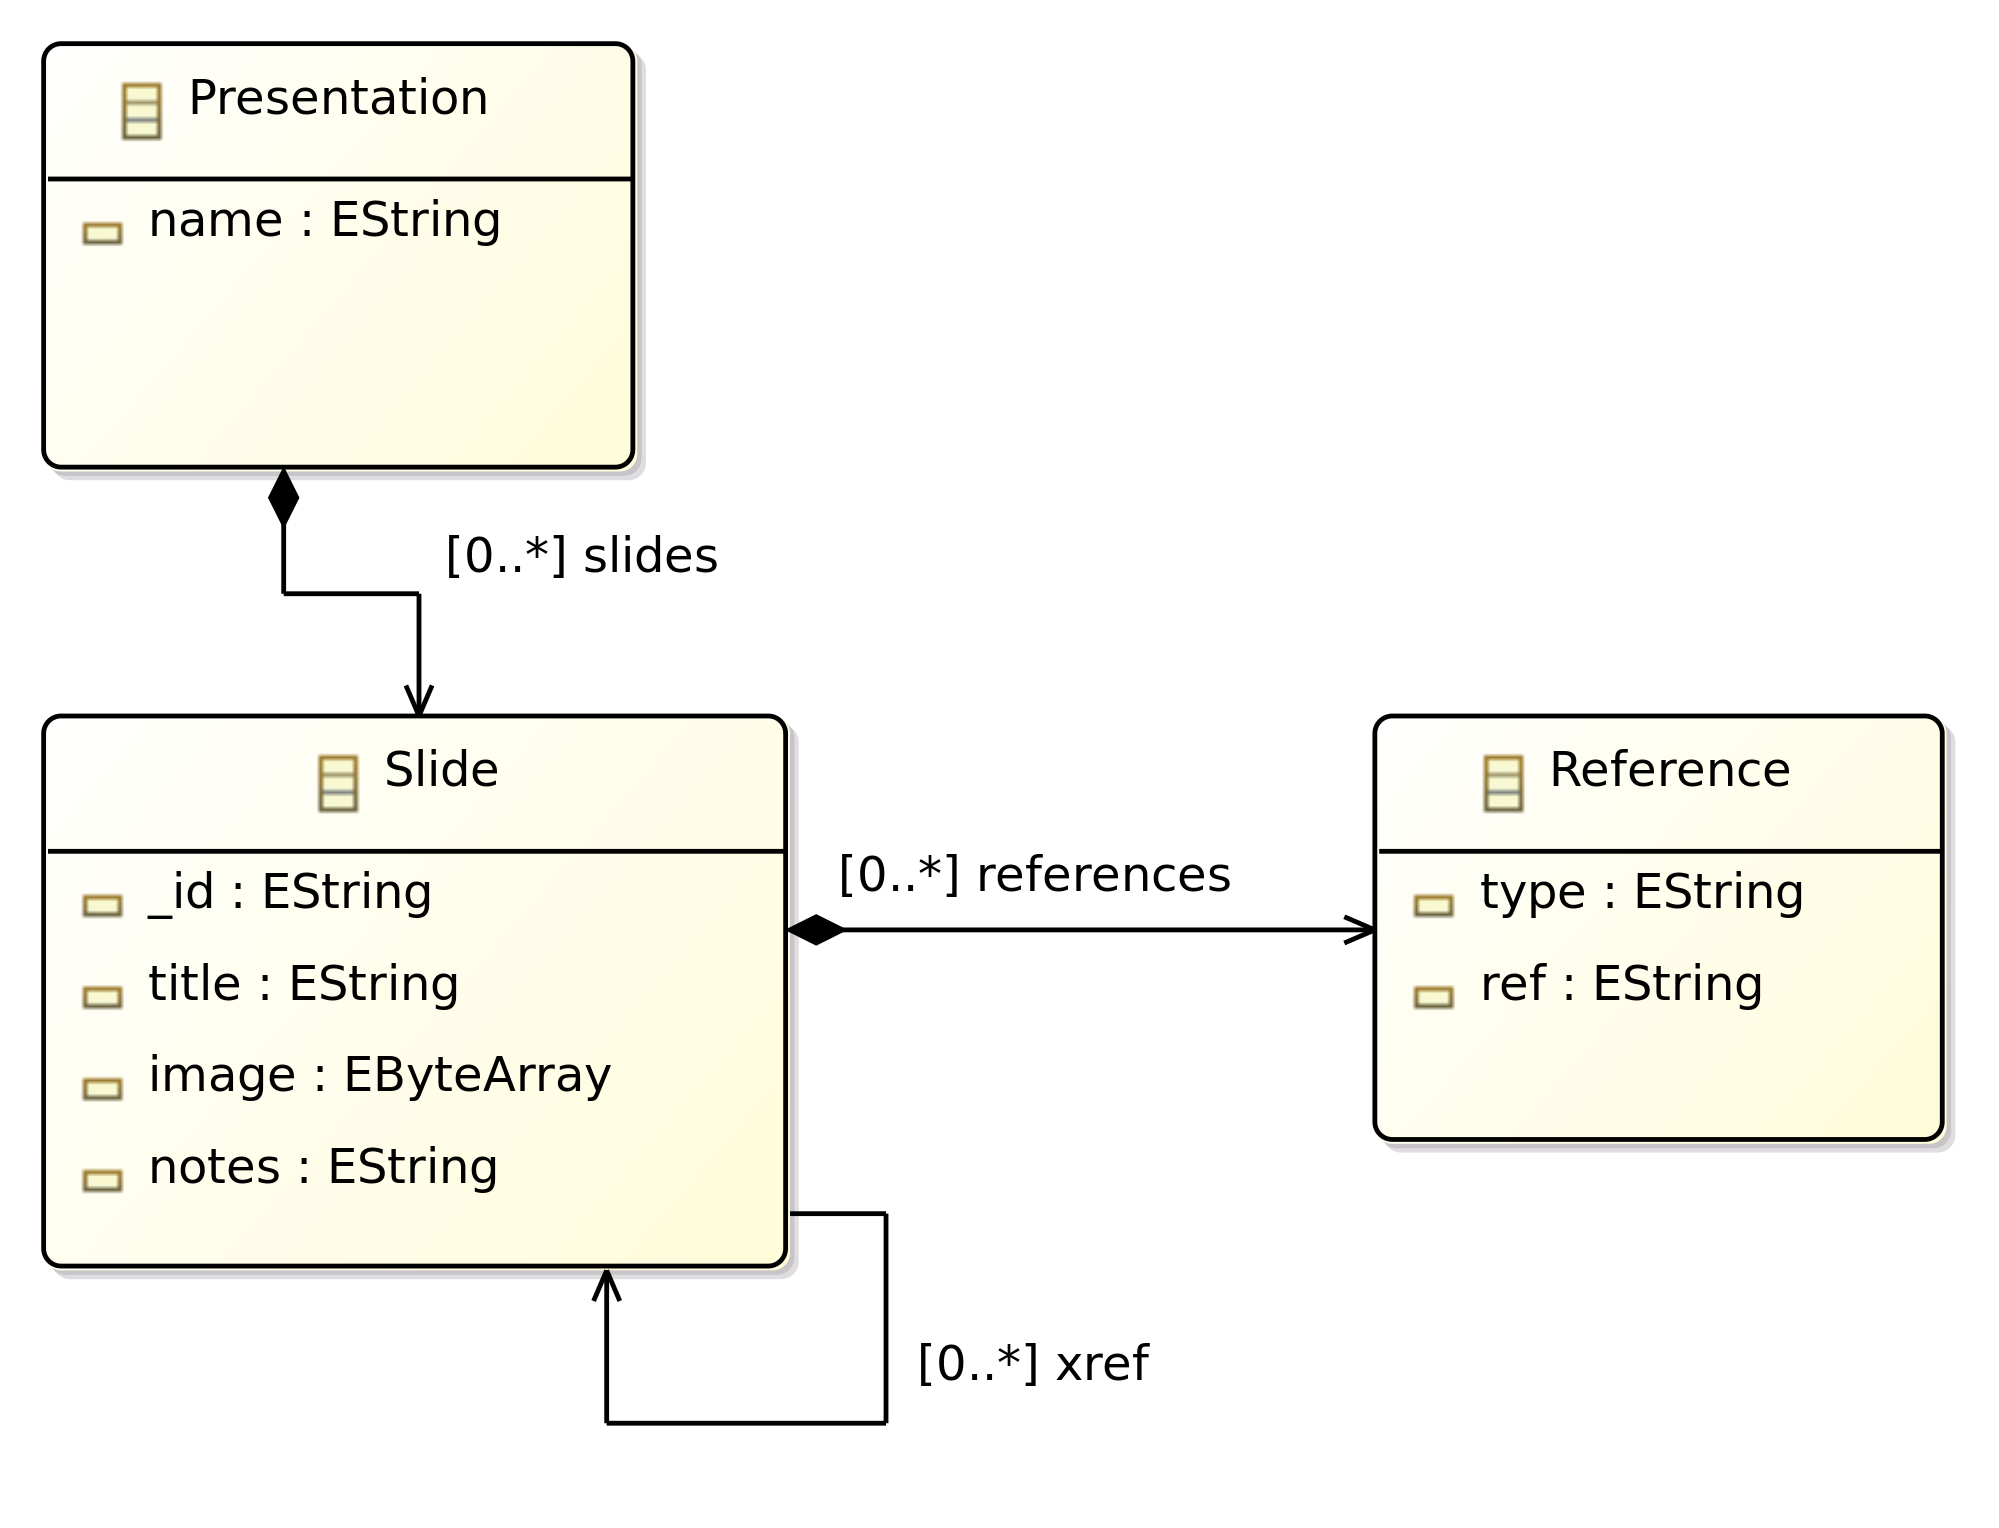
\includegraphics[width=.9\textwidth]{img/slides-data-model}

\framebreak

\begin{itemize}
\item OK, pensemos en {\bf relacional}
  \begin{itemize}
  \item \lstinline[language=sql]{CREATE TABLE ...}
  \item ¿Cuántas tablas?
  \item Claves ajenas, restricciones de integridad...
  \item {\bf Gap semántico}:
    \begin{itemize}
    \item La tabla {\tt Reference} no está contenida {\bf sino enlazada}
      (por clave ajena)
    \item O bien se crea la tabla {\tt Slide\_Reference}
    \item {\bf ID Artificial} para referencias
    \item Se tiene que crear la tabla {\tt Slide\_xref}
    \end{itemize}
  \end{itemize}

\end{itemize}

\begin{block}{El modelo de documentos es {\bf más natural en este caso}}
\end{block}

\framebreak

\begin{alertblock}{¿Y toda la información de diapositiva?}
\begin{itemize}
\begin{lstlisting}[language=sql]
SELECT * FROM Slides WHERE `_id` = 'slide000';
\end{lstlisting}
  \item ¿{\tt xref}? ¿{\tt references}?
\begin{lstlisting}[language=sql]
SELECT * FROM Slides s
  JOIN References r ON `s._id` = r.slide_id
  JOIN Slide_xref x ON `s._id` = x.slide_id
WHERE `s._id` = 'slide000';
\end{lstlisting}
\item Filas con {\bf ¡¡información replicada!!}
\item ¿Y si se añade más información a {\tt Slide}?
  \end{itemize}
\end{alertblock}

\framebreak

\begin{block}{MongoDB}
\begin{lstlisting}[language=Python]
slide = slides.find_one({'_id': 'slide000'})
\end{lstlisting}
\end{block}

\end{frame}


\section{Introducción a los sistemas NoSQL}

\begin{frame}
  \frametitle{Introducción a NoSQL}
\begin{itemize}
% \item Sobre los \~{}2010s, se renueva la búsqueda de la escalabilidad, con
%   el abaratamiento del {\em hardware}
% \item Se {\bf diversifican los problemas}, la inclusión del {\bf análisis
%     de todos los datos disponibles por parte de las empresas}
% \begin{itemize}
% \item incluso de algunos que no se había pensado usar, p. ej. {\em
%     clickstreams\/}), {\bf publicidad a la carta}, etc.
% \end{itemize}
\item {\bf NoSQL} \ra{} {\em hashtag\/} llamativo que se
  eligió para una conferencia en~2009 (Johan Oskarsson de Last.fm)
\item Ahora se asocia a cientos de bases de datos diferentes,
  que se han clasificado en varios tipos (las veremos después),
  caracterizadas por {\bf no usar SQL} como modelo de datos
\item {\bf NoSQL} \ra{} {\bfseries\itshape Not Only SQL} (no sólo SQL)
\item Big Data \ra{} hay una variedad de fuentes de datos ({\bf persistencia
    polígota})
  \end{itemize}
\end{frame}

\begin{frame}[allowframebreaks]
\frametitle{Cambio a NoSQL -- ¿Por qué?}
%En general, el desarrollo de NoSQL ha venido motivado, entre otras, por una
%serie de circunstancias:
\begin{enumerate}
\item {\bf Mayor escalabilidad horizontal}
  \begin{itemize}
  \item conjuntos de datos muy muy grandes
  \item sistemas de alto volumen de escrituras ({\em streaming\/} de
    eventos, aplicaciones sociales)
  \end{itemize}
\item {\bf Demanda de productos de software libre} (crecimiento de las {\em
    start-ups})
\item {\bf Consultas especializadas} no eficientes en el modelo relacional
  (JOINs)
\item {\bf Expresividad, flexibilidad, dinamismo}. Frustración con {\bf
    restricciones} del modelo relacional \ra{} ({\bfseries\itshape
    schemaless})
\item Paradigma {\bf funcional}: {\em Map-Reduce}
\end{enumerate}

\framebreak

\begin{alertblock}{Sin embargo...}
\begin{small}
Hay que elegir la herramienta correcta para cada aplicación, y SQL puede ser
una buena opción $\Rightarrow$ {\bf polyglot persistence}
\end{small}
\end{alertblock}
\end{frame}

\begin{frame}
  \frametitle{Introducción a NoSQL}
  \begin{block}{Categorías de NoSQL}
    \begin{itemize}
    \item Bases de datos Key-Value
    \item Bases de datos Documentales
    \item Bases de datos columnares
    \item Bases de datos de grafos
    \item Bases de datos de arrays
    \end{itemize}
\end{block}
\end{frame}


\begin{frame}
  \frametitle{Evolución desde el modelo relacional}
\begin{itemize}
\item El {\bf modelo relacional} $\Rightarrow$ {\bf predominante en los
  últimos~30~años}
\item Tiene raíces en el denominado {\em business data processing},
  procesamiento de transacciones y {\em batch}
\item Propuesto por Codd en los~70, {\bf de alto nivel}
\item Actualmente los {\bf sistemas SQL están muy optimizados}:
\begin{itemize}
\item el {\bf grado de implantación es mayoritario}
\item para el 99\% de los problemas (que caben en un ordenador) es
  eficiente y adecuado
\end{itemize}
\end{itemize}
\end{frame}

% http://db-engines.com/en/ranking/


\begin{frame}
  \frametitle{Cambio a NoSQL}
Twitter cambiando a Cassandra por~2010\\
Cassandra desarrollada en Facebook en~2009\\
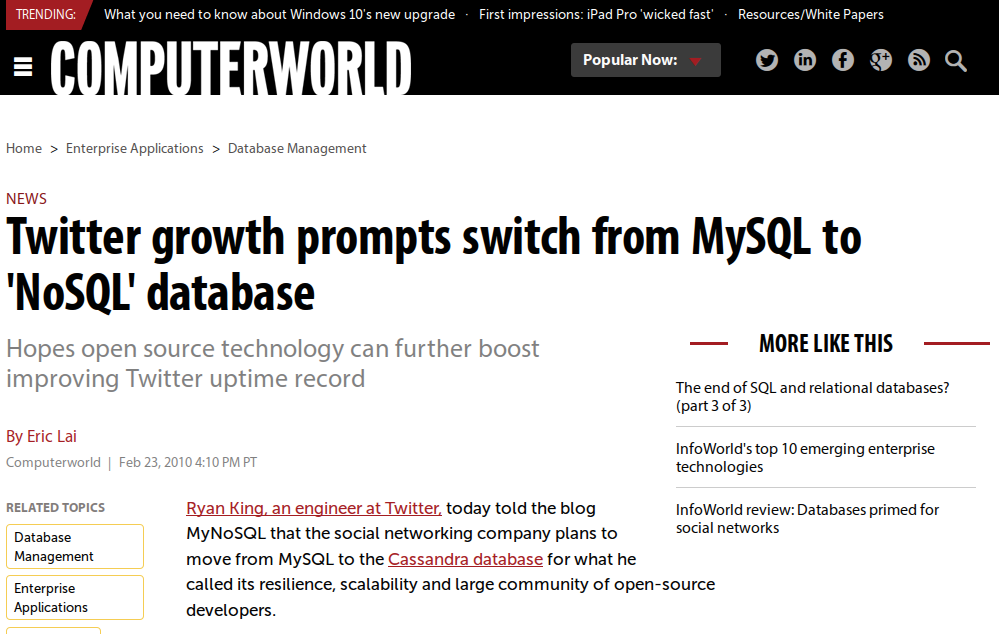
\includegraphics[width=\textwidth]{img/twitter-cassandra}
\end{frame}

\begin{frame}
  \frametitle{Cambio a NoSQL. Ranking julio 2017}
\framesubtitle{Fuente: \url{http://db-engines.com/en/ranking/}}
\vspace*{.1ex}
\centering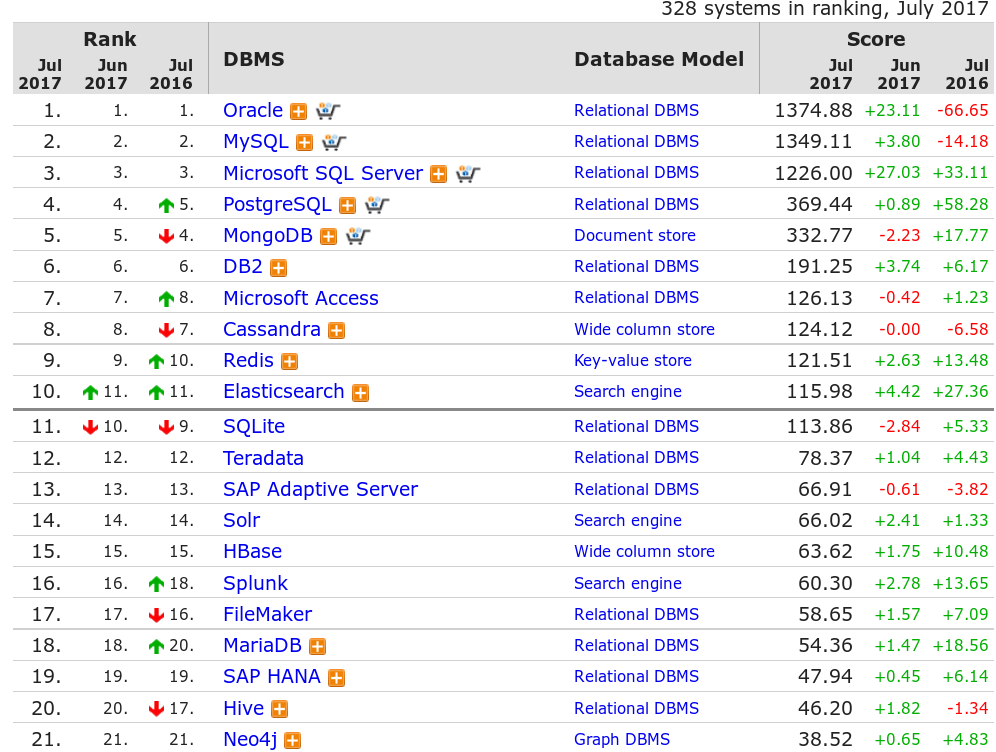
\includegraphics[width=.8\textwidth]{img/ranking-bbdd}
\end{frame}

\begin{frame}
\frametitle{Cambio a NoSQL.Tendencia julio 2017}
\framesubtitle{Fuente: \url{http://db-engines.com/en/ranking/}}
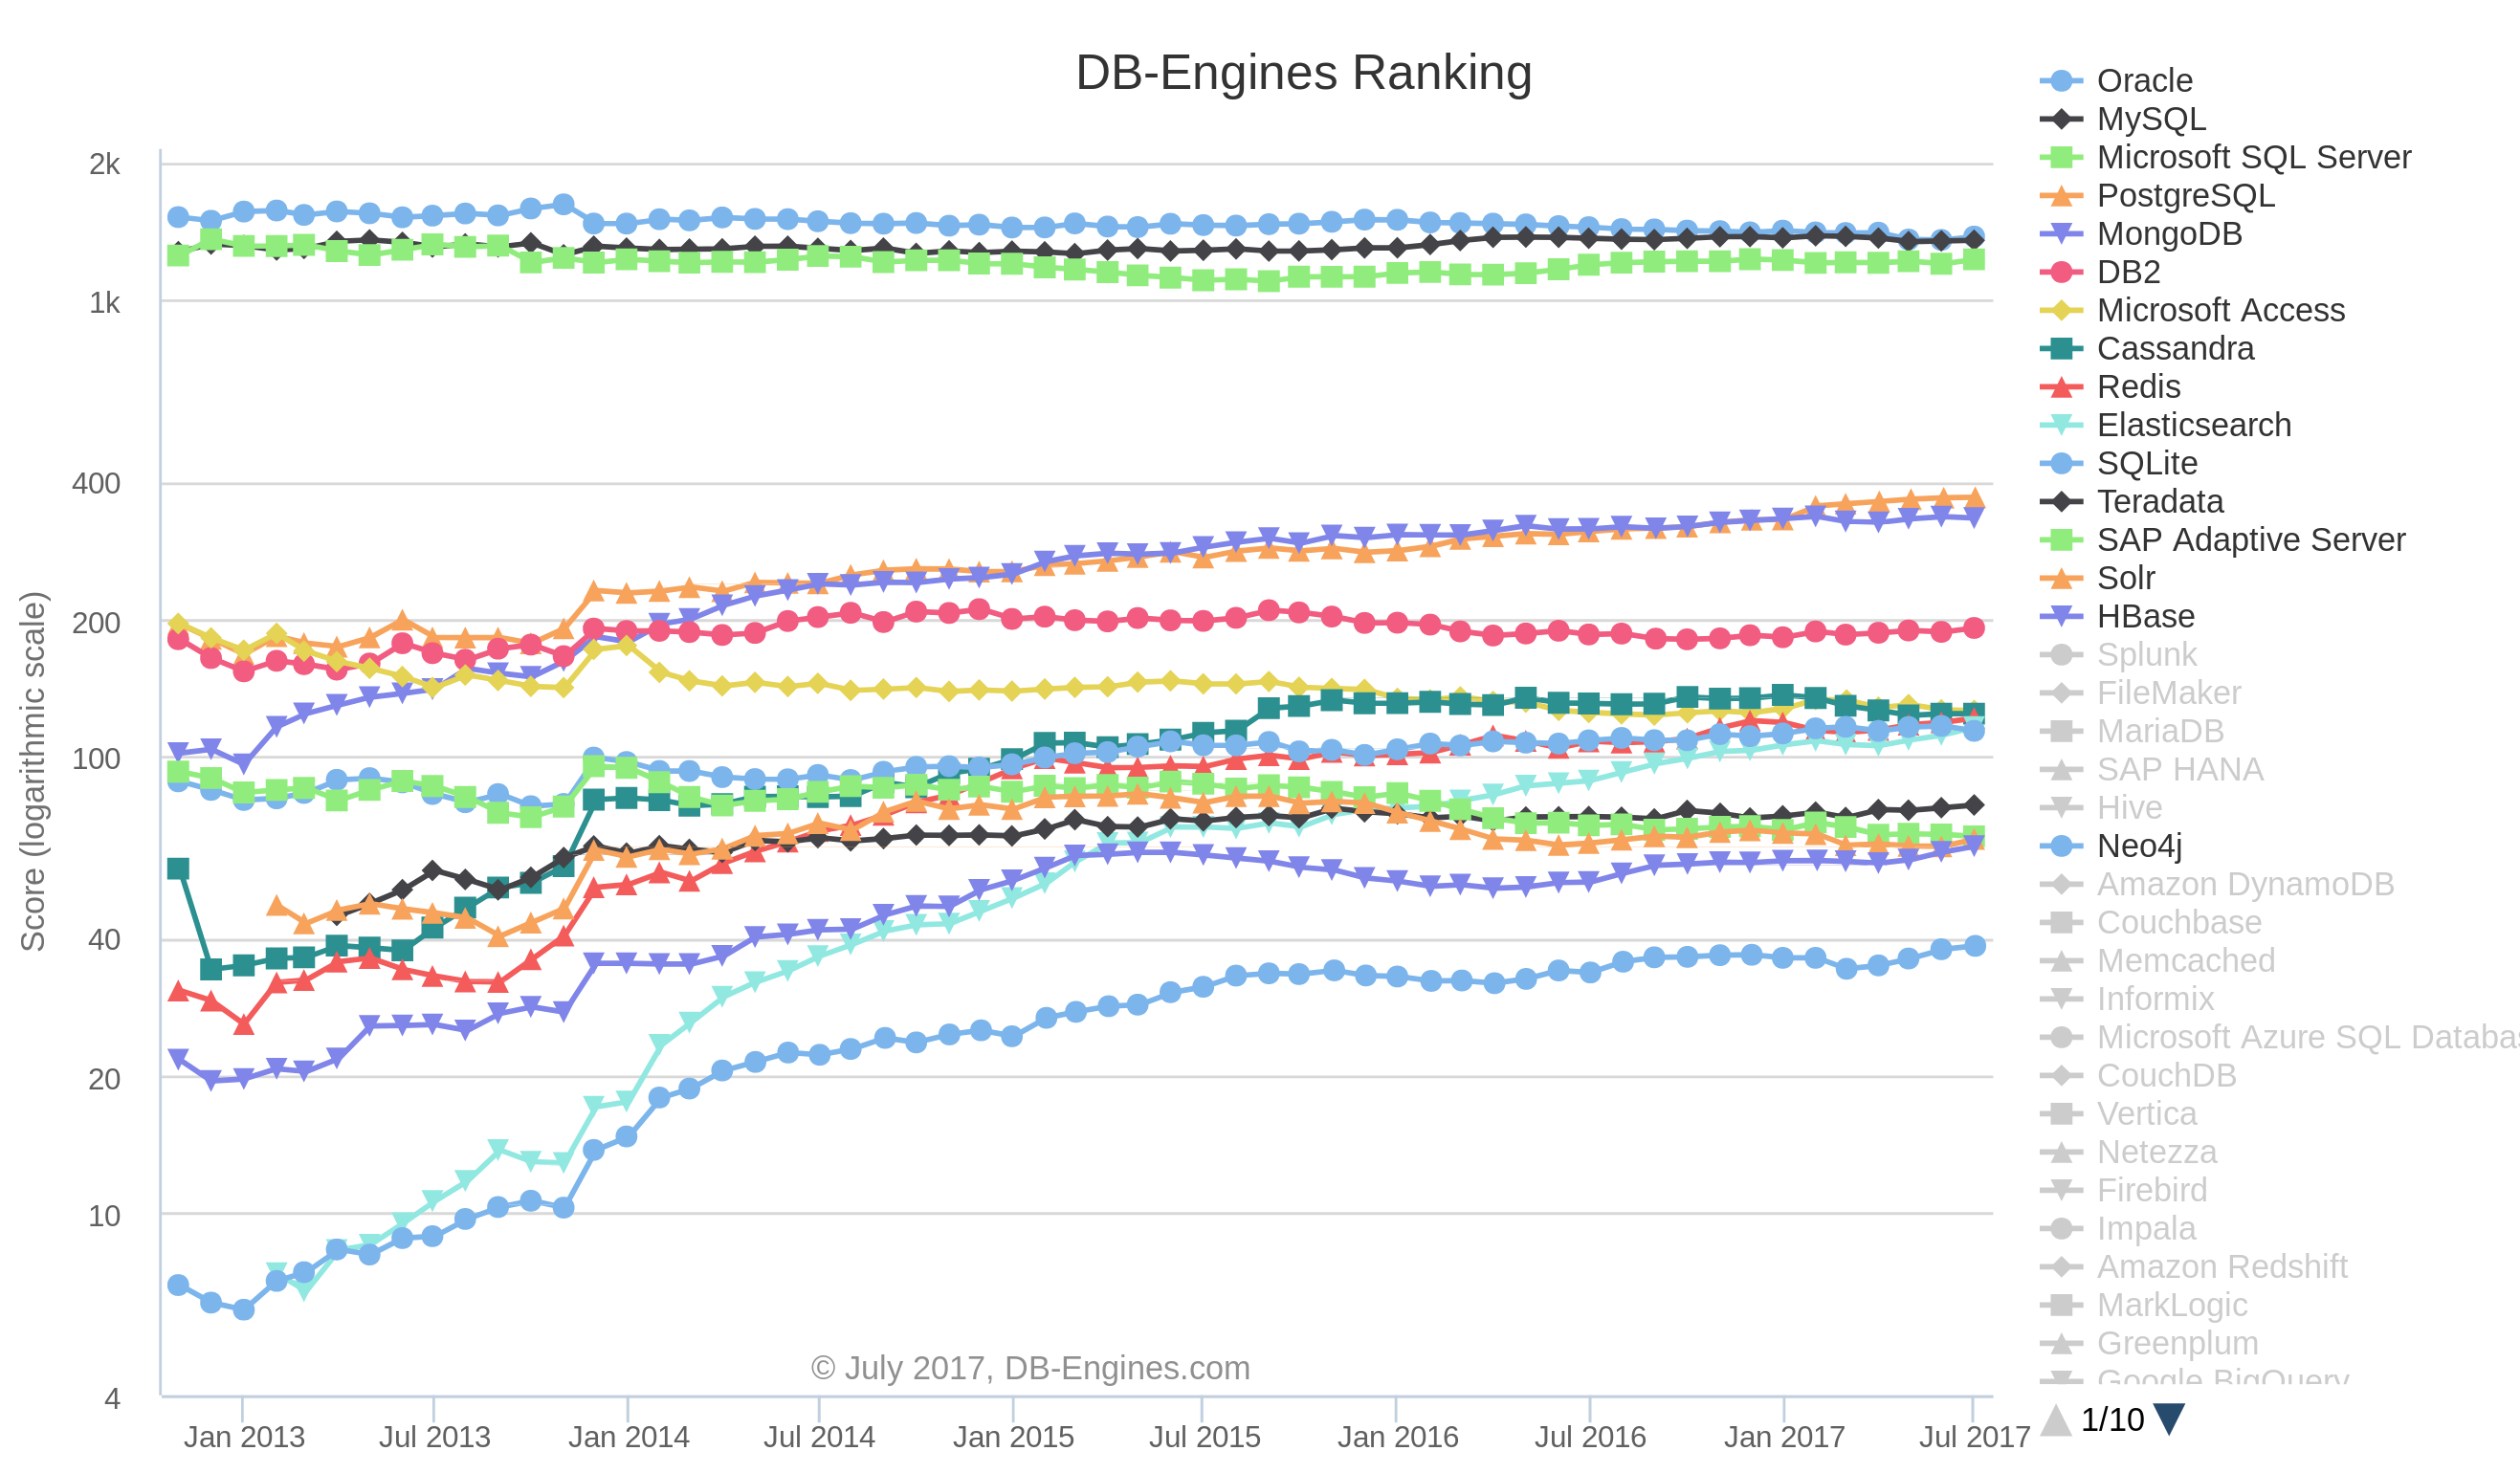
\includegraphics[width=\textwidth]{img/nosql-database-ranking}
\end{frame}

\begin{frame}
  \frametitle{Cambio a NoSQL -- Análisis}
\begin{alertblock}{Análisis}
\begin{itemize}
\item Dominan los grandes SGBDR
\item El {\em Open Source} tiene una importancia crucial (MySQL,
  MongoDB, etc.)
\item Varias bases de datos NoSQL entre las~10 primeras. Muchas en las~20
  primeras
\item La distancia entre los grandes SGBDR y el primer NoSQL (MongoDB) es
  de~5$\times$
\item Paradigmas más ``atrevidos'' como el de grafos están entre los~20
  primeros (Neo4j)
\end{itemize}
  \end{alertblock}
\end{frame}



\subsection{La importancia de la escalabilidad}

\pgfdeclareimage[height=2.7em]{sobremesa}{img/server1}%img/servidor}
\pgfdeclareimage[height=.7em]{switch}{img/switch1}%img/switch}

\newsavebox{\network}

\begin{lrbox}{\network}
\begin{tikzpicture}
  \foreach \x in {0,...,5}
    \foreach \y in {0,...,3}
    \node [] (\x\y) at (1.5*\x,1.5*\y) {\pgfuseimage{sobremesa}};

% switch
\node[inner sep=0pt] (switch) at (1.5*2.5, 1.5*4) {\pgfuseimage{switch}};

\begin{scope}[on background layer]
  \foreach \x in {0,...,5}
    \foreach \y in {0,...,3}
      \draw[gray!50] (switch)--(\x\y) ;
\end{scope}
\end{tikzpicture}
\end{lrbox}

\begin{frame}
\frametitle{Cambio de perspectiva: Red}

\begin{overlayarea}{\textwidth}{.8\textheight}
\only<1->{%
\begin{center}
\usebox{\network}
\end{center}%
}%
\only<2>{
\vspace*{-13em}
  \begin{block}{Almacenamiento distribuido}
    \begin{itemize}
    \item Desde los 90's: Clústers/NOC/COW: procesamiento masivamente
      paralelo
\end{itemize}
\begin{center}
{\color{red}SIN EMBARGO...}
\end{center}
\begin{itemize}
\item El almacenamiento no se consideraba distribuido
\item Ahora los nodos$\Rightarrow$ también para {\bf almacenamiento}
\item Se intenta minimizar el verdadero cuello de botella: {\bf trasiego de
    información por la red}
    \end{itemize}

  \end{block}%
}%
\only<3>{
\vspace*{-13em}
\begin{block}{Procesamiento distribuido}
\begin{itemize}
\item Necesidad de {\bf paralelización máxima} y {\bf escalabilidad}
\item Explotación máxima de la {\bf localidad de los datos}:
  \begin{itemize}
  \item Datos producidos se utilizan en siguientes iteraciones
\item Datos recibidos directamente (clientes simultáneos)
  \end{itemize}
\item Vuelta al modelo funcional inherentemente paralelo: (i.e. {\bf
    Map-Reduce})
\item Almacenamiento distribuido: (i.e. {\bf HDFS})
\item Coordinación distribuida: (i.e. {\bf Zookeeper})
\end{itemize}
\end{block}%
}%
\only<4>{
\vspace*{-11em}
\begin{block}{Modelo de datos}
\begin{itemize}
  \item El modelo relacional limita a tablas con valores primitivos y
    relaciones {\em Primary Key\/}/{\em Foreign Key}
  \item Pero en programación se utilizan {\bf listas}, {\bf arrays}, {\bf
      tipos de datos compuestos} ({\color{red}{\em gap\/} semántico})
  \item Además, la consistencia ACID es {\bf muy compleja y costosa} en
    ambientes distribuidos (quizá {\bf no necesaria} para algunas
    aplicaciones)
\end{itemize}
\end{block}%
}%
\only<5>{
\vspace*{-13em}
\begin{block}{Modelo de datos (ii)}
\begin{itemize}
\item ¿Y si se pudieran ver como un {\bf GRAN ARRAY}?
\begin{itemize}
\item Cada nodo almacenaría una parte del array
\item Búsqueda aleatoria {\bf muy rápida} (árboles B)
\item Búsquedas secuenciales pueden descartar nodos completos sin
  información relevante ({\bf filtros de Bloom})
\item Uso de {\bf objetos complejos} (p. ej. {\bf documentos JSON}),
  para mantener la {\bf localidad espacial de datos relacionados} (+
  después)
\item Minimización de la necesidad de transacciones: el objeto complejo es
  la unidad de {\bfseries\itshape modificación atómica}
\item Procesamiento masivamente paralelo: {\bf Map-Reduce}
\end{itemize}
\end{itemize}
\end{block}%
}%
\end{overlayarea}
\end{frame}

\subsection{Modelado de datos en NoSQL}

\begin{frame}
  \frametitle{Modelado de datos en NoSQL}
\begin{itemize}
\item El modelado de datos ({\bf en principio}) debe ser:
  \begin{itemize}
  \item Realizado al mayor nivel de abstracción posible
  \item Independiente de la tecnología subyacente
  \end{itemize}
\item Sin embargo:
  \begin{itemize}
  \item Se tiene que tener en cuenta el diseño {\bf distribuido}
  \item Se tiene que considerar qué consultas se realizan para ofrecer un
    acceso {\bf eficiente}
  \end{itemize}
% \item Para decidir la mejor tecnología de BD hay que entender las
%   relaciones entre las diferentes entidades {\bf y además} qué datos se van
%   a necesitar
%   \begin{itemize}
%   \item Por ejemplo, se preguntará ``{\bf ¿cómo diseño este conjunto de
%       tablas o este documento para esta relación uno a muchos?}''
%   \item Y también, ``{\bf ¿qué consultas se van a realizar sobre los
%       datos?}'' (las cuales van a definir cómo organizo las tablas o
%     documentos)
%   \end{itemize}
\item Con respecto al modelo de datos:
\begin{itemize}
\item Se mantienen los conceptos de entidad, relación, cardinalidades, etc.
\item El modelado relacional se centra en especificar {\bf qué datos
    tenemos y podemos ofrecer}
\item El modelo NoSQL se centra en {\bf optimizar qué
    consultas vamos a servir}
\item Es ``barato'' {\bf duplicar (desnormalizar)} los datos si con ello se
  consigue {\bf mayor eficiencia de acceso}
\end{itemize}
\end{itemize}
\end{frame}

\begin{frame}
  \frametitle{Representación relacional de un CV}
\framesubtitle{Kleppmann, 2016. \emph{Designing Data Intensive Applications}}
\vspace*{-.8ex}
  \centering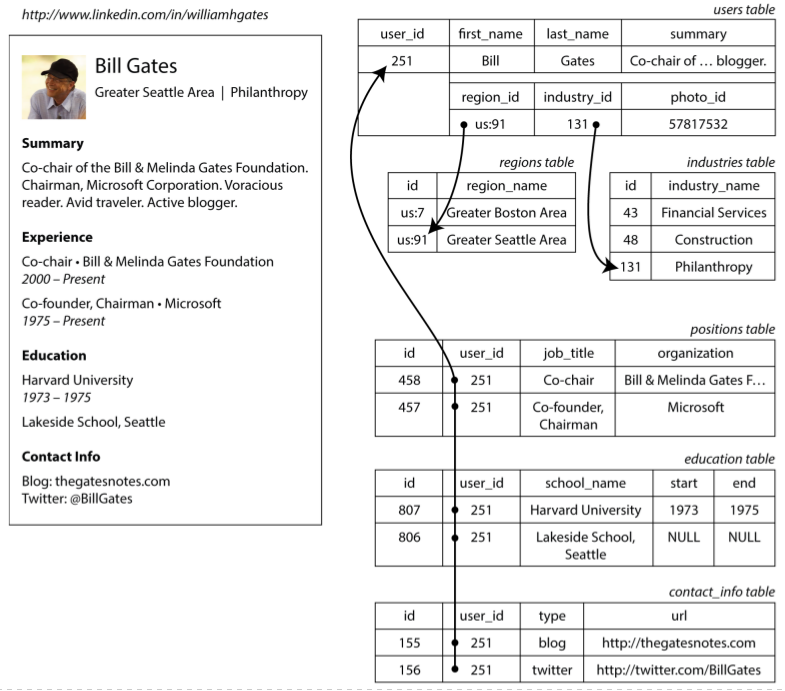
\includegraphics[height=.86\textheight]{img/gates}
\end{frame}

\begin{frame}
  \frametitle{Representación de relaciones}
\framesubtitle{Relaciones uno a muchos}
\begin{itemize}
\item Las relaciones uno a muchos (por ejemplo en el resumen: {\tt
    positions}) en el modelo relacional:
\begin{itemize}
\item Normalización usando varias tablas ({\tt Positions} con
  {\tt user\_id})
  \begin{itemize}
  \item Necesidad de más de una tabla
  \item Necesidad de uso de {\tt JOIN} $\Rightarrow$ ineficiencia
  \end{itemize}
\item Algunos SGBDR ofrecen la posibilidad de tener tipos de datos
  estructurados y campos XML o JSON. (P. ej. PostgreSQL)
  \begin{itemize}
  \item Usualmente no se pueden usar para buscar dentro
  \item No son estándar
  \end{itemize}
\end{itemize}
\end{itemize}
\end{frame}

\begin{frame}[fragile]
  \frametitle{CV como un documento}
\begin{lstlisting}[language=json,basicstyle=\tiny\tt]
{
  "user_id": 251,
  "first_name": "Bill",
  "last_name": "Gates",
  "summary": "Co-chair of the Bill & Melinda Gates... Active blogger.",
  "region_id": "us:91",
  "industry_id": 131,
  "photo_url": "/p/7/000/253/05b/308dd6e.jpg",
  "positions": [
    {
      "job_title": "Co-chair",
      "organization": "Bill & Melinda Gates Foundation"
    },
    {
      "job_title": "Co-founder, Chairman",
      "organization": "Microsoft"
    }
  ],
  "education": [
    {
      "school_name": "Harvard University",
      "start": 1973,
      "end": 1975
    },
    {
      "school_name": "Lakeside School, Seattle",
      "start": null,
      "end": null
    }
  ],
  "contact_info": {
    "blog": "http://thegatesnotes.com",
    "twitter": "http://twitter.com/BillGates"
  }
}
\end{lstlisting}
\end{frame}

\begin{frame}
  \frametitle{CV como un árbol (equivalente)}
\centering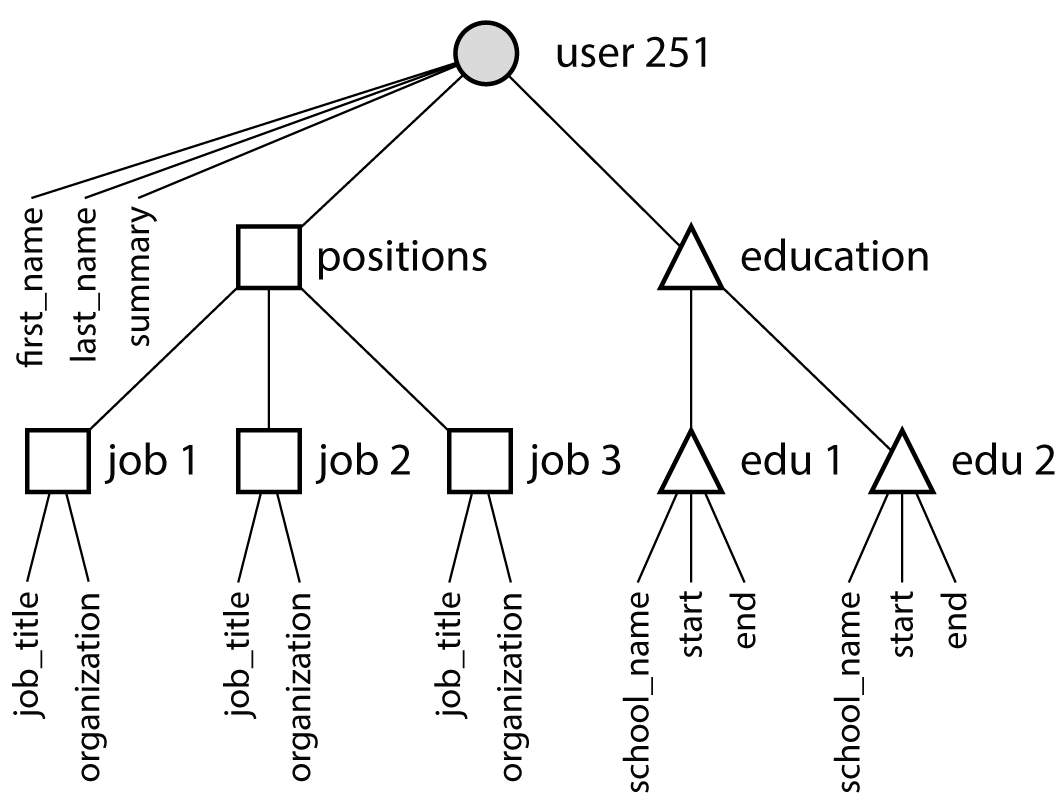
\includegraphics[height=.85\textheight]{img/tree}
\end{frame}

\begin{frame}
  \frametitle{Representación de Relaciones (ii)}
\framesubtitle{Modelo de documentos}
\begin{itemize}
\item El {\bf modelo de documentos} sigue la analogía del {\bf array/mapa
    gigante}
\item Los datos se estructuran como un {\bf conjunto de documentos}
  (objetos complejos)
\item Cada documento tiene:
  \begin{itemize}
\item Un {\bf identificador único}, con algún tipo de campo {\em id\/}
\item Este campo permite la búsqueda aleatoria eficiente por clave ({\bf
    referencia})
\item Una estructura jerárquica de sub-documentos contenidos $\Rightarrow$
  {\bf agregación}
\end{itemize}
\item Nótese que permite más flexibilidad que el modelo relacional
  (elección entre \underline{\em referencia} y \underline{\em agregación})
\end{itemize}
\end{frame}

\begin{frame}
  \frametitle{Representación de Relaciones (iii)}
\framesubtitle{Uno a muchos (ii) -- NoSQL}
\begin{itemize}
\item Relaciones {\bf Uno a Muchos} ({\tt positions}):
  \begin{itemize}
  \item {\bf Opción 1}: Agregando la tabla {\tt positions}
  \item {\bf Opción 2}: Convertir las empresas en entidades, y utilizar una
    {\bfseries\itshape referencia}
  \end{itemize}
\item ¿Qué opción elegir?
\end{itemize}
\pause
\vspace*{-.8ex}
\begin{alertblock}{¡Modelado guiado por el acceso a datos!}
\begin{small}
  \begin{itemize}
  \item Si los elementos ``muchos'' tienen una estructura sencilla
    $\Rightarrow$ {\bf Opción~1}
\item Si los elementos ``muchos'' son usualmente {\bf recuperados en una
    consulta} junto con el elemento ``uno'' $\Rightarrow$ {\bf Opción~1}
\item Si los elementos ``muchos'' son relativamente grandes, o bien son
  recuperados siempre de forma separada $\Rightarrow$ {\bf Opción~2}
  \end{itemize}
\end{small}
\end{alertblock}
\end{frame}

\begin{frame}
  \frametitle{Representación de Relaciones (iv)}
  \framesubtitle{Muchos a uno y muchos a muchos}
  \begin{itemize}
  \item Las relaciones muchos a uno y muchos a muchos:
    \begin{itemize}
    \item Personas que viven en una región
\item Preguntas que refieren a Tags
    \end{itemize}
  \item No muy adecuado al modelo de documentos
\item Al menos no aportan ventajas con respecto al modelo relacional
\item Al haber muchas entidades que refieren a otra entidad,
  la {\em agregación} daría lugar a mucha {\bf duplicación} (y a
  problemas de sincronización)
% \begin{itemize}
% \item (A no ser que las entidades sean {\bf muy pequeñas}, y se puede
%   agregar una lista $\Rightarrow$ {\tt Tags} en {\tt Post})
% \end{itemize}
\item {\color{red} $\Rightarrow$} {\bf Referencias} (sobre el ID), similar a
  una FK en el modelo relacional
  \begin{itemize}
  \item {\bf Sin embargo}, al no haber {\bf JOINs} la aplicación tiene que
    hacer más de una petición a la BD
  \end{itemize}
  \end{itemize}
\end{frame}

\begin{frame}
  \frametitle{Muchos a muchos -- referencia}
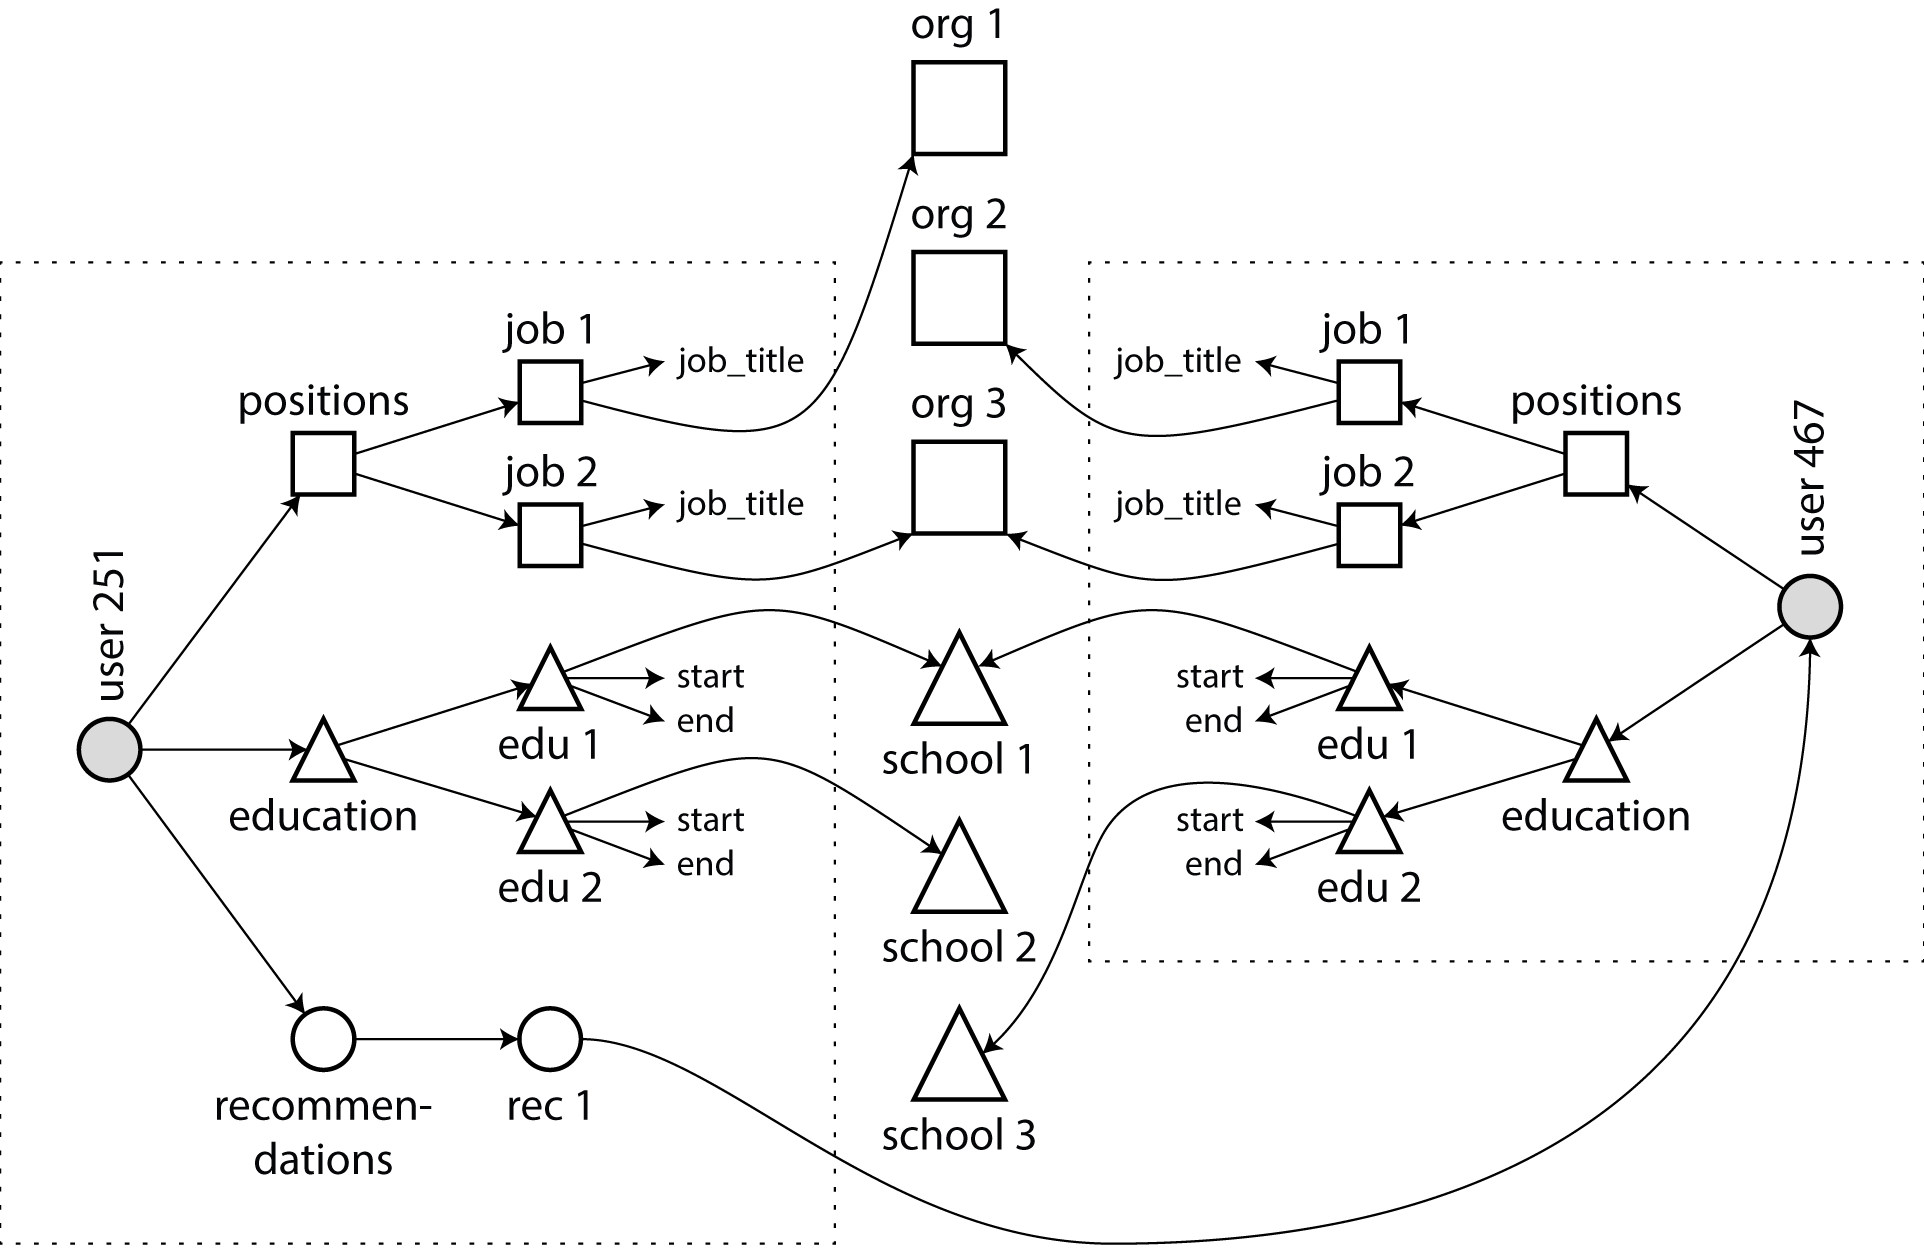
\includegraphics[width=\textwidth]{img/many-to-many}
\end{frame}

% \begin{frame}
%   \frametitle{Reconsiderando el modelo de documentos}
%   \begin{itemize}
%   \item Las ventajas del modelo basado en documentos son:
%     \begin{itemize}
%     \item Para algunas aplicaciones, la abstracción de documentos se acerca
%       más al modelo de datos
% \item La abstracción de documentos aporta más flexibilidad al esquema. Por
%   ejemplo, se pueden añadir campos diferentes a cada documento (también
%   llamados modelos {\itshape\bfseries schemaless\/})
% \item En algunos casos puede mejorar la eficiencia gracias a la localidad
%   (agregación)
%     \end{itemize}
%   \end{itemize}
% \end{frame}

\begin{frame}
  \frametitle{Schemaless}
\begin{itemize}
\item NoSQL (en general) {\bf no requiere de un esquema}
\begin{alertblock}{}
  \centering
  \href{https://farm6.staticflickr.com/5483/29931060254_109e3e36da_o_d.jpg}{\bf
    SCHEMALESS}
\end{alertblock}
\item {\bf Flexibilidad}: Posibilidad de almacenar documentos con una
  estructura diferente
\begin{itemize}
\item Tratar información incompleta
\item Evolucionar la base de datos/esquema
\item Añadir nuevas características a las aplicaciones
\end{itemize}
\end{itemize}

\begin{small}
\begin{tabular}{p{.43\textwidth}cp{.43\textwidth}}
{\bfseries\itshape schema-on-write}&$\Rightarrow$&{\bfseries\itshape
                                                   schema-on-read}\\
\hline
SQL&&NoSQL\\
Los datos conforman cuando se {\bf escriben}&&Los datos leídos conforman a
                                               un {\bf esquema implícito}\\
{\bf Tipado estricto} (estático) && {\bfseries\itshape Duck-Typing}
                                    (dinámico) \\
Datos homogéneos && Datos {\bf heterogéneos}
\end{tabular}
\end{small}
% \item Se pasa de {\em schema-on-write} (se asegura que los
%   datos son conformes cuando se escriben, como en relacional) a {\em
%     schema-on-read} (los datos tienen un {\bfseries\itshape esquema
%     implícito} cuando se leen)
% \item Así, las bases de datos NoSQL están más cerca de los lenguajes
%   dinámicos, mientras que las relacionales más cerca de los lenguajes
%   estáticos
% \end{itemize}
\end{frame}


% \begin{frame}
%   \frametitle{Schemaless (ii)}
%   \begin{itemize}
% \item El verdadero {\bf problema es: ¿cómo tratar esos datos?}
%   \begin{itemize}
% \item {\bf De manera genérica}, como almacenes de datos, o bien
%   \item Que los documentos tengan una {\bfseries\itshape variación
%       controlada}, en donde se mantienen fijos unos datos ``estándar'' del
%     tipo de documento, y se pueden añadir otros campos que, si no se
%     necesitan, se ignoran (conocido como {\bfseries\itshape duck typing})
%   \end{itemize}
%   \end{itemize}
% \end{frame}

\begin{frame}[fragile]
  \frametitle{Schemaless (ii)}
\vspace*{-.7em}
\begin{itemize}
\item {\bf Ejemplo}: En un momento se decide añadir el campo {\tt
    first\_name} a partir del campo {\tt name}
\item Se empieza a incluir objetos con el nuevo formato
\item A la hora de leerlos, se puede hacer:
\end{itemize}
\begin{lstlisting}
if (user && user.name && !user.first_name) {
   // Docs anteriores a 2013 no tienen first_name
   user.first_name = user.name.split(" ")[0];
}
\end{lstlisting}
\begin{itemize}
\item En SQL puede ser un proceso muy costoso (procesa toda la tabla, puede
  que haya que parar las aplicaciones):
\end{itemize}
\begin{lstlisting}[language=SQL]
ALTER TABLE users ADD COLUMN first_name text;
UPDATE users SET first_name =
    substring_index(name, ' ', 1);
\end{lstlisting}
\end{frame}

\begin{frame}
  \frametitle{Schemaless (iii)}
  \begin{itemize}
\item ¿Cuándo es apropiado {\em schemaless}?
  \begin{itemize}
  \item Cuando el sistema está compuesto por un número de objetos
    heterogéneos
\item Cuando la estructura de los datos está impuesta por un sistema
  externo y tenemos que ser capaces de gestionarlos
\item Si intuimos que los datos cambiarán en el futuro
  \end{itemize}
\end{itemize}
\end{frame}

\begin{frame}[fragile]
  \frametitle{Schemaless (iv)}
\begin{itemize}
\item {\bf SIN EMBARGO...} Desde un punto de vista práctico, {\bf un
    esquema es conveniente}
\item En algunos casos necesario, para facilitar el desarrollo y evitar
  inconsistencias
  \begin{itemize}
  \item {\tt Mongoose} para MongoDB permite definir esquemas:
  \end{itemize}
  \end{itemize}
\begin{lstlisting}[language=Java]
var Comment = new Schema({
  name: { type: String, default: 'Anonymous' },
  age: { type: Number, min: 18, index: true },
  bio: { type: String, match: /[a-z]/ },
  date: { type: Date, default: Date.now },
  buff: Buffer
});
// a setter with on-line modification
Comment.path('name').set(function (v) {
  return capitalize(v);
});
\end{lstlisting}

\end{frame}

\subsection{Eficiencia {\em raw}}

\begin{frame}[allowframebreaks]
  \frametitle{Eficiencia {\em raw}}
  \begin{itemize}
  \item Pero los sistemas NoSQL tienen que competir también con los SQL en
    términos de eficiencia neta (también llamada {\em raw})
  \item Un pequeño test sintético nos puede ayudar a hacernos una idea
    (fuente:
    \url{http://bonesmoses.org/2016/07/15/pg-phriday-a-postgres-persepctive-on-mongodb/}
  \item Estos resultados están también en la hoja del repositorio de la
    asignatura
    \url{https://github.com/dsevilla/bdge/blob/master/addendum/mysql_vs_mongo/perf_plot.ipynb}.

\framebreak

\item La prueba se realizó sobre MongoDB y sobre MySQL (se ha adaptado el
  original, que era para PostgreSQL)
\item Se parte de una tabla sencilla con cuatro valores, que muestran
  medidas de sensores con localización, valor de la lectura y una marca de
  tiempo
  \item Se realizan seis pruebas que pueden corresponder a un conjunto de
    consultas normales:
\framebreak
  \begin{enumerate}
  \item Inicialmente se insertan un millón de elementos generados al azar,
    con fechas que permitan la búsqueda por rango ({\bf Fill})
  \item Se crea un índice en la tabla para la fecha de la lectura ({\bf
      Index})
  \item Se actualizan los valores de un conjunto de entradas seleccionadas
    por rango de fechas ({\bf Update})
  \item Se eliminan un conjunto de filas seleccionadas por rango de fechas
    ({\bf Delete})
  \item Se obtiene el número de filas restantes ({\bf Count})
  \item Se obtiene un {\bf subconjunto} de filas extraído de una consulta
    dada por un rango de fechas ({\bf Interval})
  \end{enumerate}

\end{itemize}

\begin{center}
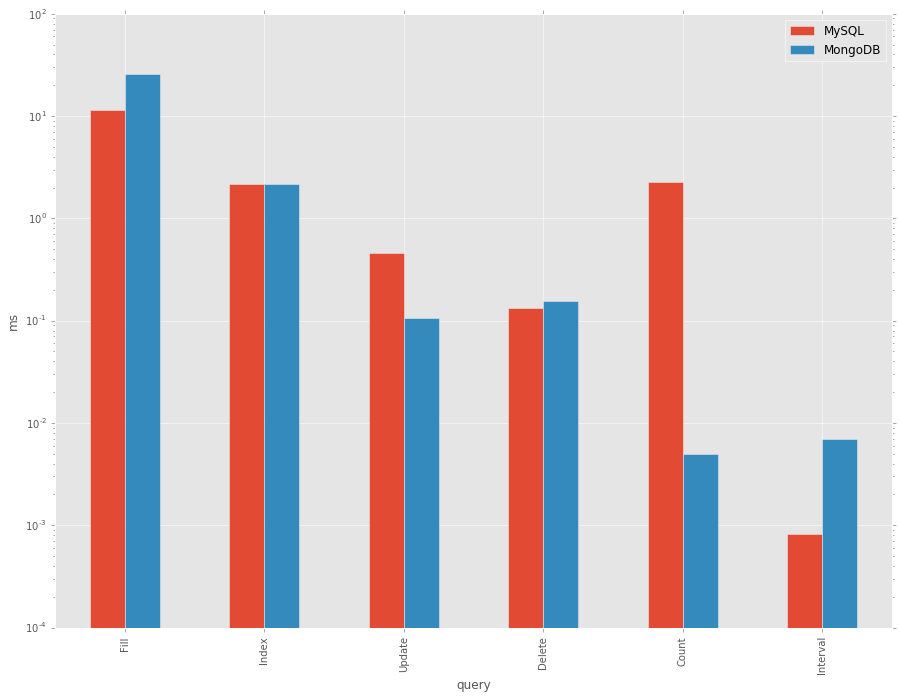
\includegraphics[width=.8\textwidth]{img/mongo_vs_mysql}
\end{center}


\begin{itemize}
\item El gráfico se muestra en escala logarítmica en el eje Y (las
  diferencias pequeñas se acentúan)
\item A simple vista, ambos productos están muy igualados
  \begin{itemize}
  \item SQL (MySQL) lleva {\em muchos años} de optimizaciones
  \item Mientras que productos como MongoDB tienen menos historia a sus
    espaldas en cuanto a optimizaciones, etc.
  \end{itemize}
\item Hay casos en los que uno es más rápido que el otro y viceversa
\item No se puede decir cuál es mejor
  \begin{itemize}
  \item {\bf $\Rightarrow$ DEPENDE DEL PATRÓN DE ACCESOS QUE VAYA A TENER
      NUESTRA APLICACIÓN}
  \item (p. ej. contado en MongoDB mucho más rápido que en MySQL;
    actualización algo más rápida)
  \end{itemize}
\end{itemize}

\end{frame}

% \begin{frame}
%   \frametitle{Map-Reduce}
% \begin{itemize}
% \item La escalabilidad de las bases de datos relacionales está limitada por
%   la ley de Moore
% \item Los {\em clústers} surgieron como una alternativa para proporcionar
%   {\em escalabilidad horizontal} (vs. escalabilidad vertical, mejorar un
%   procesador)
% \item Sin embargo, las bases de datos relacionales no casan bien con los
%   clústers ({\em joins} en tablas muy grandes, tablas temporales, etc.)
% \item Como se ha dicho, las bases de datos NoSQL surgieron como una
%   respuesta a estas limitaciones
%   \begin{itemize}
%   \item Al preferir la {\bf agregación} (localidad) a la referencia (claves
%     ajenas), cada entidad almacenada se hace más independiente
% \item Por lo tanto, se puede almacenar de forma más sencilla en un {\em
%     pool} de servidores
% \item Se adoptó también el paradigma funcional de procesamiento de datos
%   $\Rightarrow$ {\bf Map-Reduce}
% \item Millones de máquinas ejecutan {\bf en paralelo procesos} sobre datos
%   que están {\bf físicamente distribuidos}, alojando los resultados {\bf
%     localmente en cada servidor} (descentralización, HDFS, Hadoop, etc.)
%   \end{itemize}
%   \end{itemize}
% \end{frame}

\section{Tipos de Sistemas NoSQL}


\subsection{Key-Value y Documentales}

\begin{frame}
  \frametitle{Key-Value Stores y Documentales}
  
\includegraphics[width=\textwidth]{img/MongoDB}
\end{frame}

\begin{frame}
  \frametitle{Key-Value Stores y Documentales}
\vspace*{-.9em}
\begin{itemize}
\item Cada pieza de datos tiene asignado un identificador
\item La diferencia entre ambas es que:
  \begin{itemize}
  \item En Key-Value, el valor es opaco, no se conoce nada de su interior
    (a todos los efectos es un {\em blob\/} de datos)
\item En las basadas en documentos, la base de datos puede ver el contenido
  del agregado, y utilizar su información como parte de las búsquedas y
  actualizaciones
\end{itemize}
\item Docs. $\Rightarrow$ formatos jerárquicos tipo JSON o XML
\item La diferencia entre ambas queda un poco difusa
  \begin{itemize}
  \item Por ejemplo, Riak es Key-Value pero permite realizar búsquedas
    indexadas parecidas a las de Solr/Lucene
\item Redis permite que los valores de datos sean estructurados en arrays,
  estructuras complejas, mapas
  \end{itemize}
\item Key-Value: Riak, Redis, Memcache, LevelDB
\item Documentos: CouchDB, MongoDB, OrientDB
\end{itemize}
\end{frame}

\subsection{Map-Reduce}

\begin{frame}[allowframebreaks,fragile]
\frametitle{Map-Reduce}
\begin{itemize}
\item Origen en {\bf lenguajes funcionales}:
\begin{itemize}
\item {\tt map()}: Ejecuta una misma función sobre todos los elementos de
  un conjunto
\begin{lstlisting}[language=haskell]
map :: (a -> b) -> [a] -> [b]
\end{lstlisting}
\item {\tt reduce()}: Procesa un conjunto de valores para producir un
  valor de salida
\begin{lstlisting}[language=haskell]
foldl :: (a -> b -> a) -> a -> [b] -> a
\end{lstlisting}
\end{itemize}

\framebreak

\item Map-Reduce combina ambas operaciones:
\begin{itemize}
\item Una misma operación {\tt map()} a cada dato residente en un nodo es
  realizada de forma paralela en {\bf todos} los nodos simultáneamente
\item Con los resultados parciales de cada nodo, una función {\tt reduce()}
  genera un resultado (o un conjunto de resultados) final
\item Hay un proceso intermedio de {\em shuffle} para agrupar valores
  relacionados antes del {\tt reduce()}
\item Resultados parciales en el mismo nodo (localidad) $\Rightarrow$
  procesamientos {\bf en cadena}
\end{itemize}
\end{itemize}

\framebreak

\centering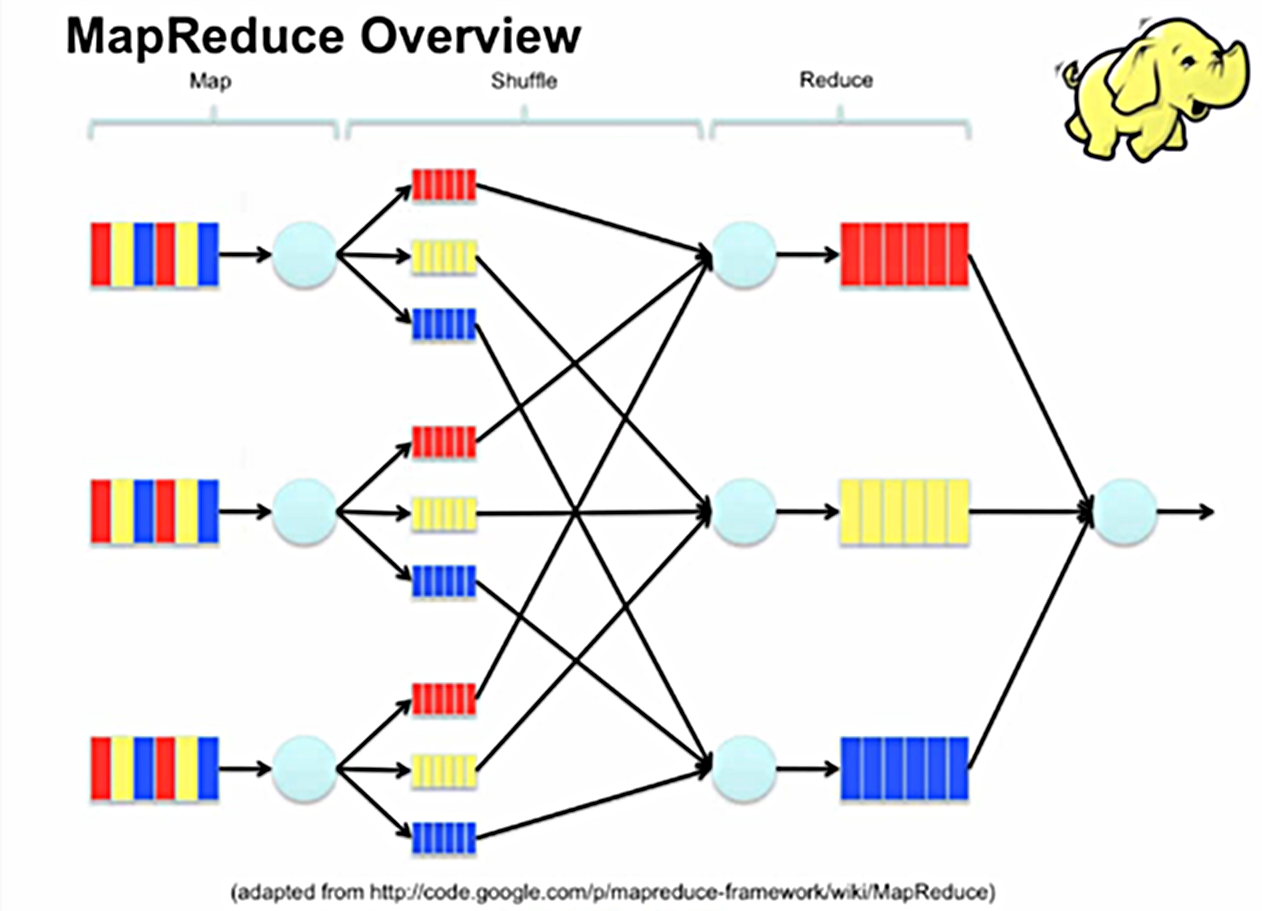
\includegraphics[width=.9\textwidth]{img/mapreduce1}

\framebreak

(de \url{http://www.milanor.net/blog/an-example-of-mapreduce-with-rmr2/})
\centering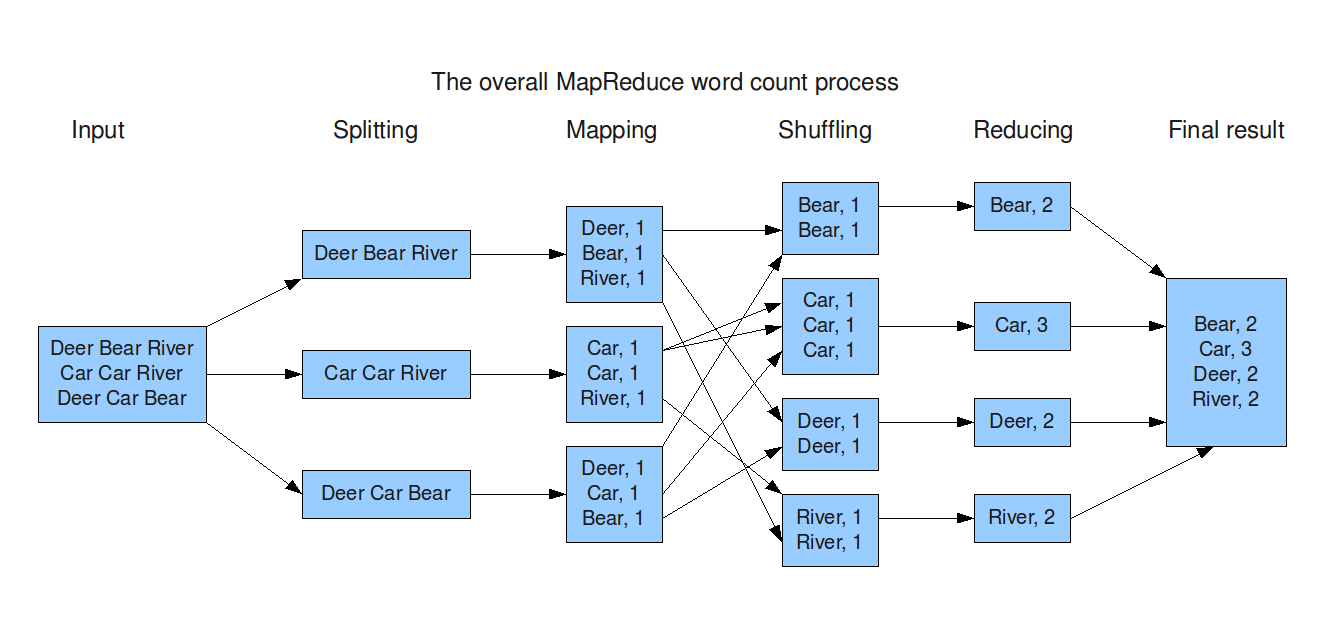
\includegraphics[width=\textwidth]{img/MapReduceWordcount}
\end{frame}

\begin{frame}
\frametitle{Map-Reduce}
\begin{itemize}
\item Map-Reduce en entornos Big-Data/NoSQL
  \begin{itemize}
  \item Entrada \ra{} siempre pares $<key,value>$

  \item {\tt map()} produce otro conjunto de valores
    $\{<key1,value1>,<key2,value2>,...\}$

\item {\em Shuffle} agrupa los valores con la misma clave:
\begin{displaymath}
\{<key1,\{val1,val3,...\}>,<key2,\{val2,val4,...\}>,...\}
\end{displaymath}

\item {\tt reduce()} procesa cada lista de valores con la misma clave, y
  produce otros elementos $<key',value'>$

\item Hay procesamientos difíciles de expresar en Map-Reduce $\Rightarrow$
  varias operaciones M/R {\bf en cadena}
  \end{itemize}
\end{itemize}
\end{frame}


\begin{frame}[fragile,allowframebreaks]
  \frametitle{Map-Reduce y Consultas}
\begin{itemize}
\item Map-Reduce puede usarse no sólo para computación distribuida, sino
  también como una {\bf generalización de consultas}
\item Ejemplo: Imagínese un biólogo marino que hace anotaciones de cada
  animal que ve en el océano, y quiere saber cuántos tiburones ha visto por
  mes:
\begin{lstlisting}[language=SQL]
SELECT MONTH(observation_timestamp) AS observation_month,
       sum(num_animals) AS total_animals
FROM observations
WHERE family = 'Sharks'
GROUP BY observation_month;
\end{lstlisting}

  \framebreak

\item MongoDB con el API de MapReduce:
\begin{lstlisting}[language=Javascript,basicstyle=\footnotesize\tt]
db.observations.mapReduce(
  function map() {
    var year = this.observationTimestamp.getFullYear();
    var month = this.observationTimestamp.getMonth() + 1;
    emit(year + "-" + month, this.numAnimals);
  },
  function reduce(key, values) {
    return Array.sum(values);
  },
  {
    query: { family: "Sharks" },
    out: "monthlySharkReport"
  }
);
\end{lstlisting}

\item  MongoDB ofrece además un API alternativo para funciones de agregación:

\begin{lstlisting}[language=Javascript,basicstyle=\footnotesize\tt]
db.observations.aggregate([
  { $match: { family: "Sharks" } },
  { $group: {
    _id: {
       year: { $year: "$observationTimestamp" },
       month: { $month: "$observationTimestamp" }
    },
    totalAnimals: { $sum: "$numAnimals" }
  }
  }
]);
\end{lstlisting}
\end{itemize}
\end{frame}

\begin{frame}[plain]
  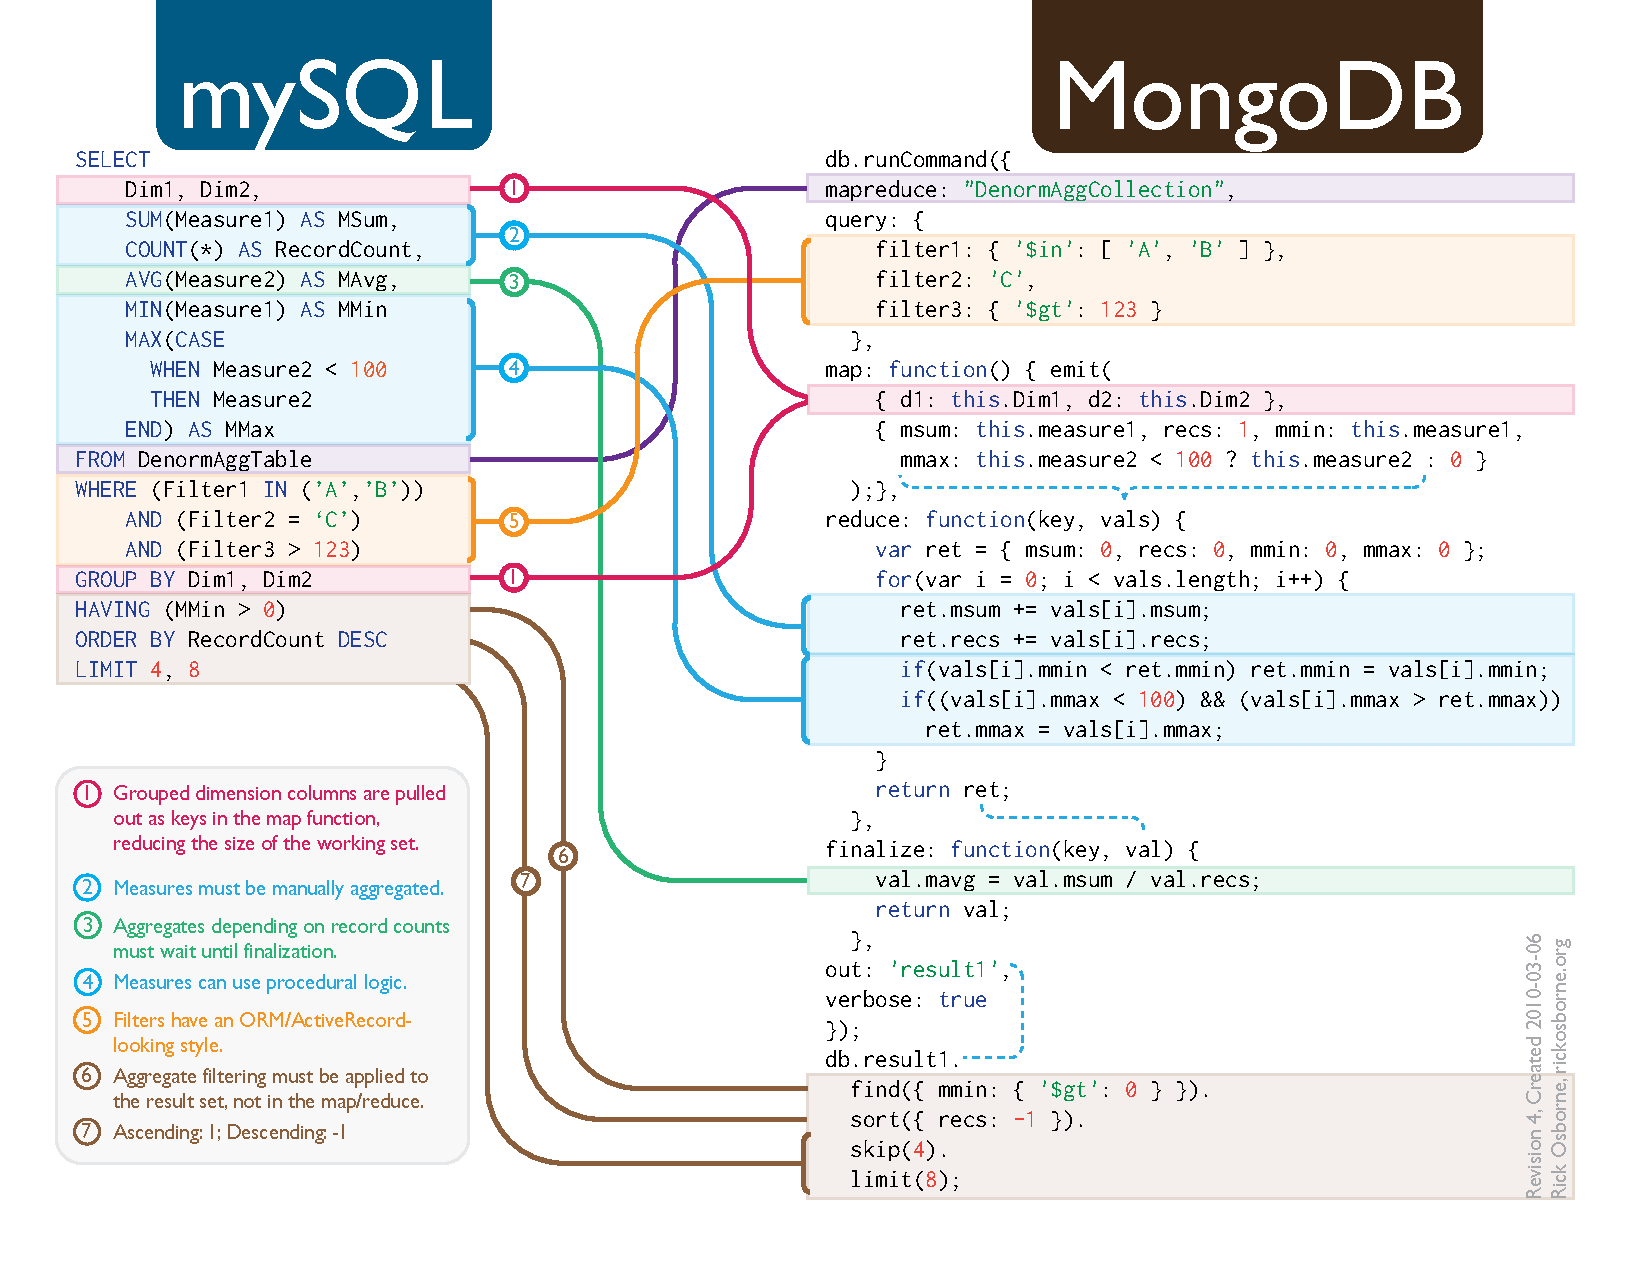
\includegraphics[width=\textwidth]{img/sql-to-mongodb}
\end{frame}

\end{document}


\subsection{Bases de Datos Columnares}

\begin{frame}
  \frametitle{Bases de Datos Columnares}
\begin{itemize}
\item Influenciadas por el Paper de Google de 2004 sobre BigTable
\item En general, parecidos a las tablas SQL, salvo que cada fila puede:
  \begin{itemize}
  \item Tener un conjunto de columnas diferente
\item Almacenar {\em series temporales} dentro de una misma fila (varias
  {\em versiones} de un mismo conjunto de columnas)
  \end{itemize}
\item Cada fila tiene un identificador y es un agregado de familias de
  columnas ({\em column family})

\item Cambian el modo de almacenamiento para favorecer ciertas aplicaciones
  (almacenamiento por columnas en vez de por filas)
\item Bases de datos: HBase, Cassandra, Vertica, H-Store
\end{itemize}
\end{frame}

\begin{frame}[plain]
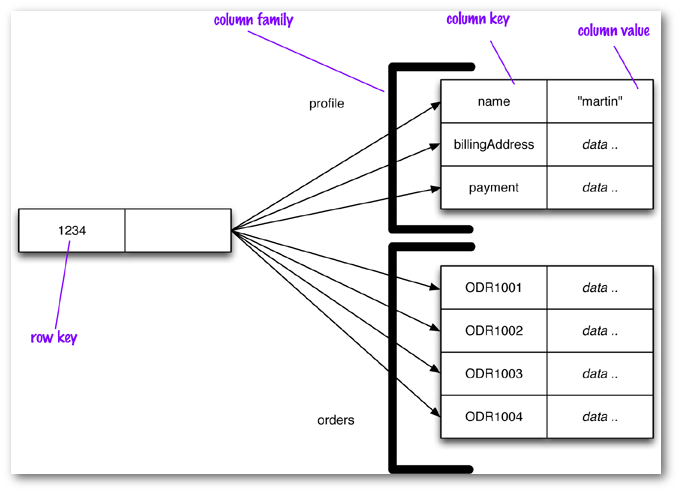
\includegraphics[width=\textwidth]{img/column}
\end{frame}

\subsection{Bases de Datos de Grafos}

\begin{frame}
  \frametitle{Bases de Datos de Grafos}
\vspace*{-1ex}
  \begin{itemize}
  \item Las bases de datos de grafos llevan el mecanismo {\em muchos a
      muchos} al extremo
\item Datos en los que existen muchas relaciones entre sí y
  tienen un significado primordial
\item Las bases de datos de grafos se basan en la construcción y consulta
  de un grafo que consta de
  \begin{itemize}
  \item {\bf Vértices}, también llamados {\em nodos} o {\em entidades}, y
  \item {\bf Aristas} ({\bfseries\itshape Edges}), también llamados {\em
      relaciones}
  \end{itemize}
\item Los grafos pueden capturar relaciones complejas entre
  entidades y ofrecen lenguajes de búsqueda, actualización y creación que
  permiten trabajar con subconjuntos del grafo
% \item Orígenes en las bases de datos de hechos (con lenguajes de consulta
%   lógicos (p. ej. {\em Datalog})
\item Origen en las bases de datos de hechos ({\em Datalog\/})
\item Ejemplos: FlockDB, Neo4J, OrientDB
\end{itemize}
\end{frame}

\begin{frame}[plain]
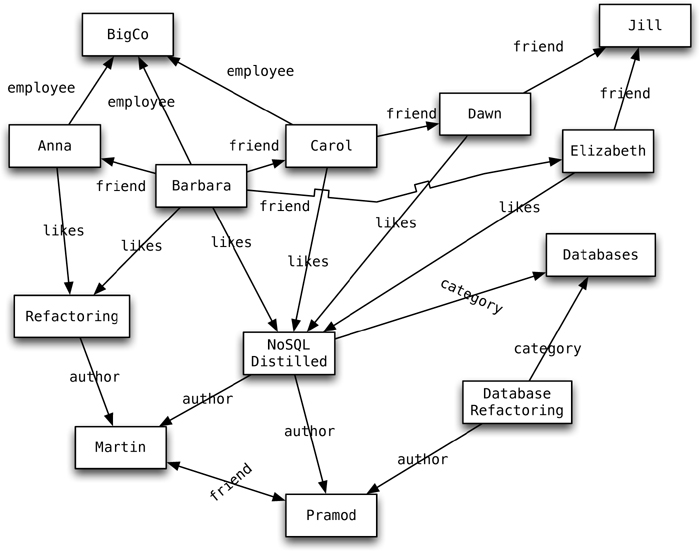
\includegraphics[width=\textwidth]{img/graph}
\end{frame}

\begin{frame}[fragile,plain]
(Nota: Usa la sintaxis PostgreSQL para {\tt json})
\begin{lstlisting}[language=SQL]
CREATE TABLE vertices (
  vertex_id integer PRIMARY KEY,
  properties json
);

CREATE TABLE edges (
  edge_id integer PRIMARY KEY,
  tail_vertex integer REFERENCES vertices (vertex_id),
  head_vertex integer REFERENCES vertices (vertex_id),
  label text,
  properties json
);

CREATE INDEX edges_tails ON edges (tail_vertex);
CREATE INDEX edges_heads ON edges (head_vertex);
\end{lstlisting}
\end{frame}

\begin{frame}[fragile]
  \frametitle{Ejemplo de datos y consulta en Neo4J}
\vspace*{-1.5ex}
\begin{block}{}
\begin{lstlisting}
CREATE
  (NAmerica:Location {name:'North America', type:'continent'}),
  (USA:Location {name:'United States', type:'country' }),
  (Idaho:Location {name:'Idaho', type:'state' }),
  (Lucy:Person {name:'Lucy' }),
  (Idaho)-[:WITHIN]->(USA)-[:WITHIN]-> (NAmerica),
  (Lucy) -[:BORN_IN]-> (Idaho)
\end{lstlisting}
\end{block}
Y de consulta:
\begin{block}{}
\begin{lstlisting}
MATCH
(person) -[:BORN_IN]-> () -[:WITHIN*0..]-> (us:Location {name:'United States'}),
(person) -[:LIVES_IN]-> () -[:WITHIN*0..]-> (eu:Location {name:'Europe'})
RETURN person.name
\end{lstlisting}
\end{block}
\end{frame}

\subsection{Arrays}

\begin{frame}
  \frametitle{Bases de Datos basadas en Arrays}
  \begin{itemize}
\item Suelen presentarse como bases de datos que soportan SQL y añaden
  operaciones para trabajar con conjuntos de datos especiales (arrays)
\item Utilizadas para tratamiento de grandes cantidades de datos de forma
  estadística o de modelado y OLAP
\item Soportan también datos geográficos, ya que pueden definir rangos
  numéricos de una o varias dimensiones (2D para cálculos geográficos)
\item Ejemplos: MonetDB, SciDB, rasdaman
  \end{itemize}
\end{frame}

\end{document}

%%% Local variables:
%%% mode: LaTeX
%%% TeX-master: t
%%% ispell-local-dictionary: "spanish"
%%% fill-column: 75
%%% TeX-parse-self: t
%%% TeX-auto-save: t
%%% End:
%%% vim: expandtab shiftwidth=2 tabstop=2
